\documentclass{beamer} 
\usepackage{amsmath,amssymb,amsthm} 
\usepackage{pb-diagram}
\usepackage{ucs} \usepackage[utf8x]{inputenc}
\usepackage[russian]{babel}
\usepackage{graphicx}
\usepackage{multicol}

%\pagestyle{plain}

\theoremstyle{definition} \newtheorem{Def}{Definition}
\setbeamertemplate{caption}[numbered]
\newcommand{\tr}{\hat\triangleright} \newcommand{\trc}{\triangleright}
\newcommand{\adk}{a^{\dagger}_{\kappa}} \newcommand{\ak}{a_{\kappa}}
\def\bF{\mbox{$\overline{\cal F}$}} \def\F{\mbox{$\cal F$}}

\usetheme{AnnArbor}
\title[Affine Lie algebra computations]{Computational tools for representation theory of affine Lie algebras}
\author{Anton Nazarov}
\institute[SPbSU]{
  Department of high-energy physics\\
  Saint-Petersburg State University}

\date[ACSM 2009] % (optional, should be abbreviation of conference name)
{Workshop on Advanced Computer Simulation Methods for Junior scientists, April 2009}
\begin{document}
\maketitle
\begin{frame}{Outline}
  \tableofcontents
  % You might wish to add the option [pausesections]
\end{frame}

\section{Representation Theory}
\label{sec:repr-theory}
\begin{frame}{Lie Algebras}
  \begin{Def}
    {\bf Lie algebra} --- linear space $g$ with Lie bracket $ \left[ \ \right]:g\times g \to g $
  \end{Def}
  \pause 
  \begin{itemize}
  \item Why Lie algebras are interesting?
    \begin{itemize}
      \pause 
    \item Infinitesimal version of continuous symmetry groups
      \pause 
    \item Connected with different areas of mathematics: differential equations, geometry, topology etc
      \pause
    \end{itemize}
  \item Classification of finite dimensional algebras
    \pause
  \item Several ways to extend the classification to infinite-dimensional Lie algebras
    \pause
  \item Affine Lie algebras --- the simplest class of infinite-dimensional Lie algebras
    \begin{itemize}
    \item Play major role in conformal field theory
    \item Are connected with modular forms
    \item Can be constructed starting from simple finite-dimensional Lie algebras
    \end{itemize}

  \end{itemize}

\end{frame}
\begin{frame}{Representations}
  \begin{Def}
    {\bf Representation} --- homomorphism from Lie algebra to linear operators on some linear space
  \end{Def}
  \begin{itemize}
  \item In physics we are interested in representations
  \item The representations can be constructed in regular way
    \begin{itemize}
    \item Integrable highest weight representations
      \begin{equation}
        \label{eq:1}
        \begin{split}
          & E^{\alpha}\left|\mu\right>=0\\
          & E^{-\alpha}\left|\mu\right>=\left|\mu-\alpha\right>\\
          & L^{\mu}=\bigoplus_{\nu\in P} V^{\nu}\\
        \end{split}
      \end{equation}
    \item The problem is to calculate weight multiplicities (subspace dimensions)
    \end{itemize}
  \item Branching --- view the representation of algebra as the sum of representations of sub-algebra
  \end{itemize}
\end{frame}
\section{Algorithms}
\label{sec:algorithms}
\begin{frame}{Main Formulae}
  \begin{itemize}
  \item Recurrent relation for weight multiplicities
    \begin{equation}
      \label{eq:2}
      mult(\xi)=-\sum_{w\in W\backslash e}det(w)\;mult(\xi+\rho-w\rho)+\sum_{w\in W}det(w)\delta_{\xi,w(\mu+\rho)-\rho}
    \end{equation}
  \item Branching of representation to representations of sub-algebra
    \begin{equation}
      \label{eq:4}
      L_{\frak{g}\downarrow \frak{a}}^{\mu }=\bigoplus\limits_{\nu \in P_{\frak{a}%
        }^{+}}b_{\nu }^{\left( \mu \right) }L_{\frak{a}}^{\nu }
    \end{equation}
    \begin{equation}
      \label{recurrent-relation}
      k_{\xi }^{\left( \mu \right) }=\frac{-1}{s\left( \gamma _{0}\right) }\left(
        \sum_{w\in W}\epsilon \left( w\right) \delta _{\xi ,\pi _{\frak{a}}\circ
          \left( w\circ (\mu +\rho )-\rho \right) +\gamma _{0}}+\sum_{\gamma \in
          \Gamma _{\frak{a}\subset \frak{g}}}s\left( \gamma +\gamma _{0}\right) k_{\xi
          +\gamma }^{\left( \mu \right) }\right)   
    \end{equation}
    \begin{equation}
      \label{eq:5}
      b_{\nu }^{\left( \mu \right) }=k_{\xi }^{\left( \mu \right) } \text{ for }\nu\text{ in main Weyl chamber}
    \end{equation}
  \end{itemize}
\end{frame}
\begin{frame}{Illustration}
Computation of weight multiplicities of level 1
representation of algebra $A_1$
  \begin{figure}[bh]
  \noindent\centering{
  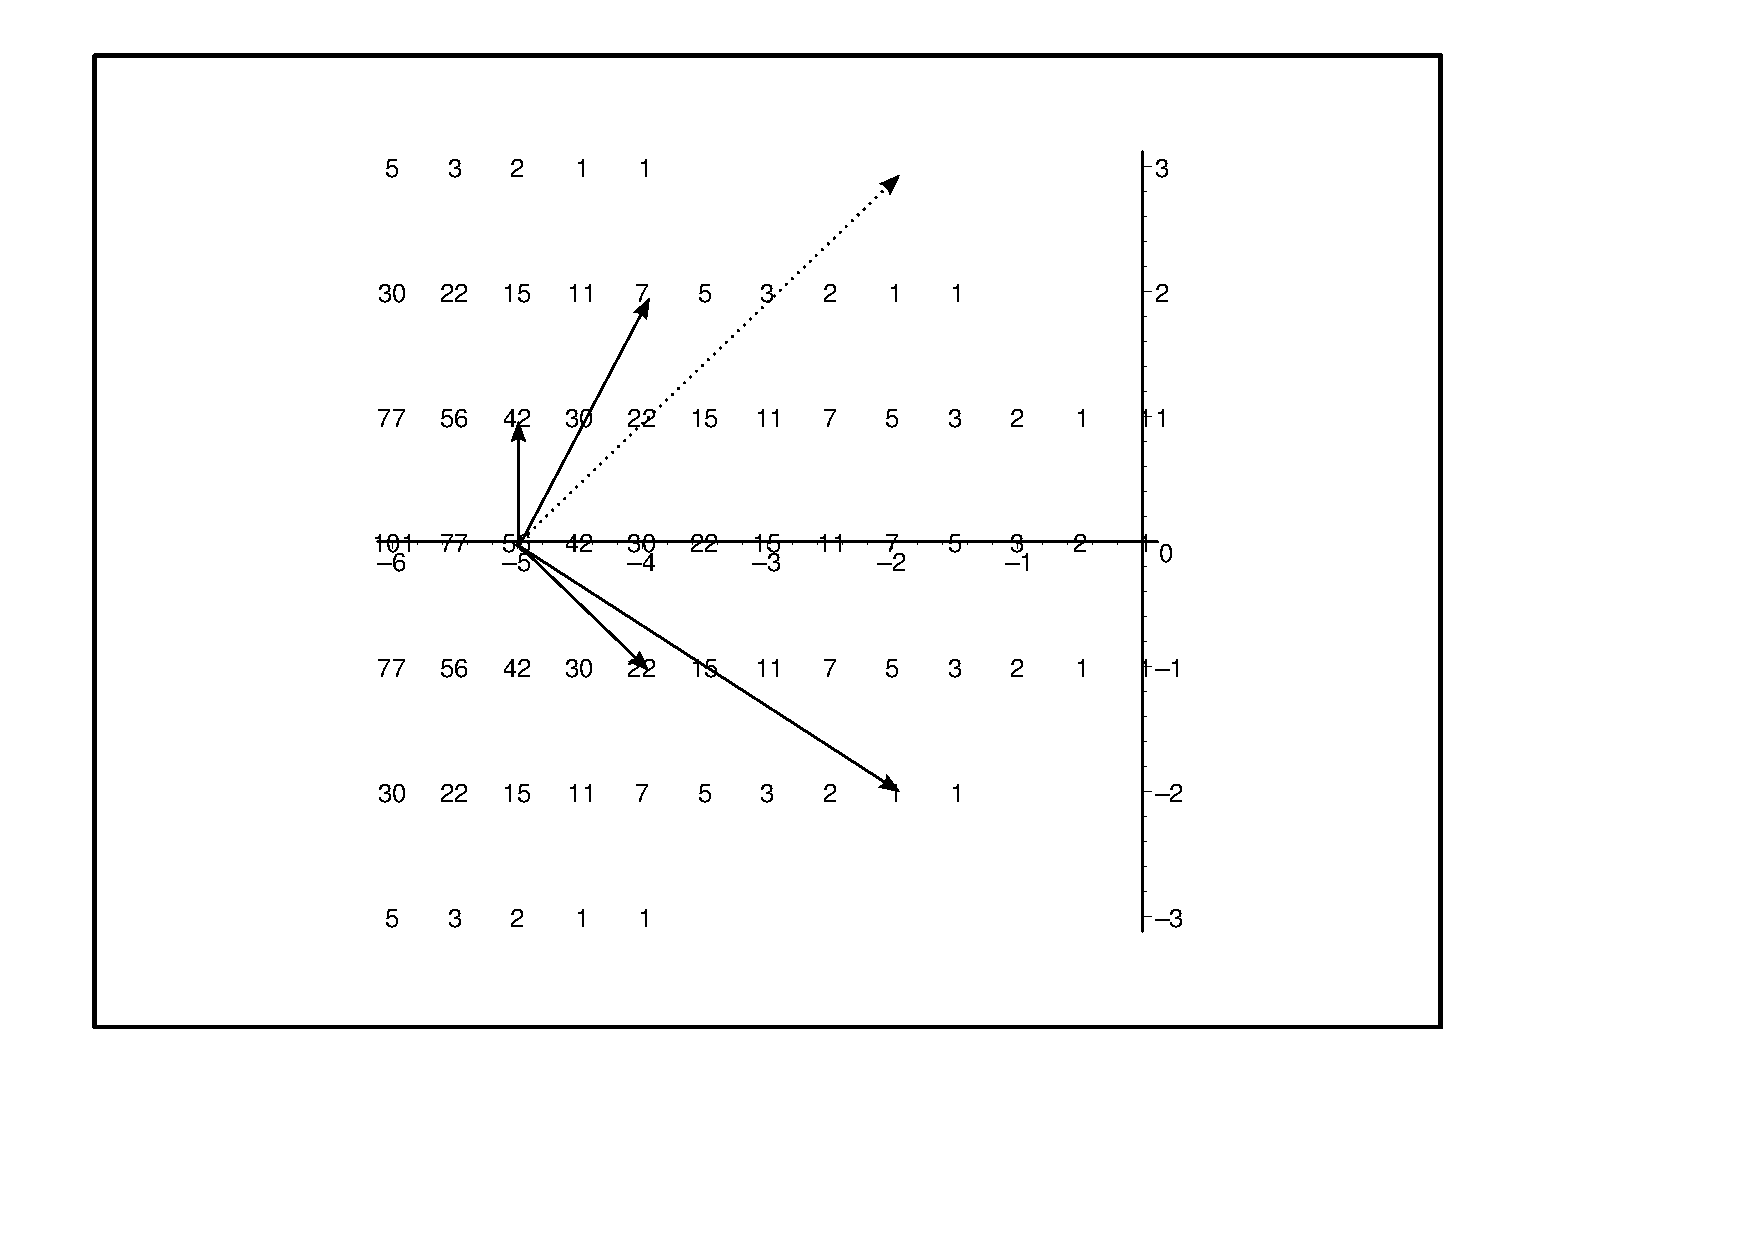
\includegraphics[width=110mm]{A1_with_star.pdf}
  }
  \label{A1 with star}
\end{figure}

\end{frame}
\section{Implementation}
\label{sec:implementation}
\begin{frame}{Maple Package}
  \begin{itemize}
  \item Based upon Coxeter/Weyl package which is very useful for finite dimensional Lie algebras\\
    \url{http://www.math.lsa.umich.edu/~jrs/maple.html}
  \item For untwisted $A_n,B_n,C_n,D_n$ and twisted $A_n^{(2)},D_n^{(2)}$ series of affine Lie algebras
    \begin{itemize}
    \item Explicit construction of
      \begin{itemize}
      \item algebra roots
      \item fundamental and dominant weights
      \item Weyl reflections
      \end{itemize}
    \item Computation of
      \begin{itemize}
      \item weight multiplicities
      \item branching coefficients for affine sub-algebra
      \end{itemize}
    \end{itemize}
  \item Freely available from my homepage \url{http://anton.nazarov.name/affine}
  \end{itemize}
\end{frame}
\begin{frame}[fragile]
  \frametitle{Examples}
  \begin{itemize}
  \item Weight multiplicities of level 2 representation of $A_3$ with highest weight $\alpha_1+\alpha_2+\alpha_3$
\begin{verbatim}
> al:=algebra_roots(A3);
      al := [e2 - e1, e3 - e2, e4 - e3, delta + e1 - e4]
> mu:=2*lambda0+sum(al[i],i=1..3);
      mu := -e1 + e4 + 2 lambda0
> string_function(mu,mu,A3,30);
[1, 7, 32, 117, 371, 1063, 2819, 7029, 16660, ...
\end{verbatim}
  \item Branching functions of module $L^{[1,0,0]}$ of $A_2$ to sub-algebra $A_1$ 
\begin{verbatim}
> tt1:=branching_rules(wg[-1],A2,A1,{e1=alpha[1]},15);
> tt1[lambda0];
           2      3      4       5       6       7 
1 + q + 2 q  + 5 q  + 7 q  + 11 q  + 17 q  + 25 q  + ...
> tt1[lambda0+e1/2];
         2      3      4       5       6       7   
2 q + 2 q  + 4 q  + 6 q  + 10 q  + 14 q  + 24 q  + ...
\end{verbatim}
  \end{itemize}


\end{frame}
\section{Summary}
\label{sec:summary}
\begin{frame}{Summary}
  \begin{itemize}
  \item The algorithms for representation theory of affine Lie algebra were presented
  \item Maple implementation was described
  \item \url{http://anton.nazarov.name/affine}
  \end{itemize}
  \vskip0pt plus.5fill
  \begin{itemize}
  \item
    Outlook
    \begin{itemize}
    \item
      Expand the code to cover affine extensions of exceptional Lie algebras
    \item
      Add the algorithms for computations for physical models of conformal field theory
    \end{itemize}
  \end{itemize}
\end{frame}

\bibliography{article}{}
\bibliographystyle{utphys}

\end{document}
